\chapter{Term Indexing}
%In automated theorem proving there are, generally, many inference rules available while only a handful few are applicable to the current subgoals. Therefore, we are interested in efficient storage of terms, both in regards to memory consumption and retrieval of generalisations and unifiables of a query term. Term indices are a category of data structures built for this express purpose.

A term index efficiently stores terms while also providing efficient operations for the retrieval of variants\footnote{Identical up to variable identity}, instances, generalisations and unifiables of a query term from the term index. Depending on the exact data structure, we can also implement other operations efficiently if desired, for example checking if a term is already stored, only inserting a term if no more general term is stored and efficiently merging two indices. In this thesis we limit ourselves to these operations as it is difficult to predict the exact use cases.

As generally presented in literature, term indices provide efficient, but overapproximating, queries. We disregard variable identities as it is prohibitively expensive to track the exact substitution while traversing the tree. By disregarding variable identities, we assume that each variable is unique and, as a result, avoid the occurs check. As such, a term index can only be used as a pre-filter whose results must, when necessary, be further filtered. We additionally disregard types as we expect the user of the index to only store consistent and type correct terms. Specifically, we assume that the arity of a function is fixed.

In the following sections we give an overview of path indexing and discrimination trees. We also take a closer look at some details of their implementation in Isabelle/ML as they differ in many places significantly from the approaches chosen in most literature.

\section{Path Indexing}
Instead of storing a term as a tree of functions and their arguments, we can specify the structure and symbols of a tree by combining every symbol of a term with its position, which we call its path.
\begin{defn}
  The path is a sequence of $(symbol, index)$ pairs where the index describes the index of the next argument to traverse.\footnote{This is in contrast to coordinate indexing which only uses a sequence of indices.}
\end{defn}
For example, the term $f(x,g(a,b))$ can be represented by a set of paths and their associated symbol as can be seen in \cref{termpaths}.
The paths always start at the root and end with the index at which the symbol is located, e.g. $<(f,2), (g,1)>$ is the path of the symbol $a$. We represent a path by enclosing a sequence of $(symbol, index)$ pairs with $<>$.

We disregard the identity of variables as they are mostly irrelevant to the queries and simplify both the index and the queries. Consequently, the terms $f(x,y)$ and $f(x,x)$ are both saved as $f(*,*)$. This leads to an overapproximation in some cases, for example $f(c,d)$ would be identified as an instance of $f(x,x)$.

\begin{defn}
  $Symbol_{t}(p)$ refers to the symbol associated with path $p$ in the term $t$.
\end{defn}

\begin{figure}[h]
\centering
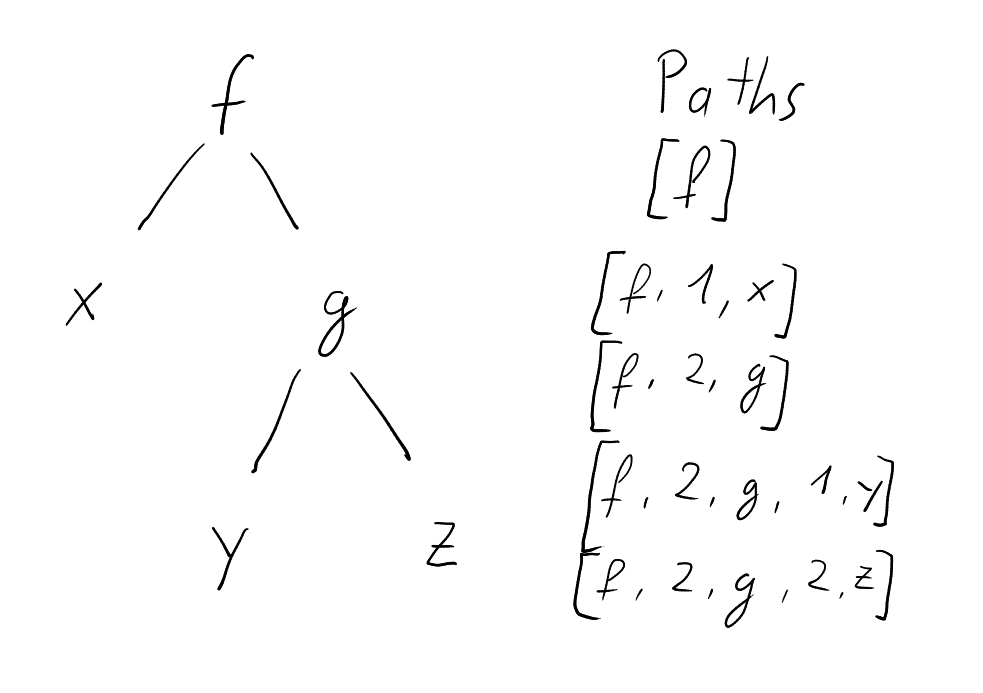
\includegraphics[scale=0.25]{figures/term_path.png}
\caption{A term and its paths together with the symbols associated with them}
\label{termpaths}
\end{figure}\todo{Figure: Write as mapping: $<> \longrightarrow f$ etc.}

A $(path, symbol)$ pair can be interpreted as a constraint on a term where the path defines the position of the symbol in the term. For example, $(<(f,1)>, c)$ is only fulfilled by terms of the form $f(c,...)$\footnote{The paths do not explicitly encode any information about the number of arguments.}. A term gives raise to a set of $(path, symbol)$ pairs, which, when interpreted as constraints, uniquely identify this term up to loss of variable identitification.

These constraints allow us to define terms not explicitly by their structure and symbols but rather by imposing constraints on them. This concept is fundamental to path indexing which stores only the constraints. Queries are resolved by combining the constraints to retrieve a set of terms.\todo{Better phrasing}

\begin{defn}
  A path index is a function $f: Path \times Symbol \longrightarrow 2^{Term}$, that is, each constraint is mapped to a set of terms, which fulfill these constraints and are stored in the path index. We call this set of terms a path set.\todo{Drop ``path set'' completely?}
\end{defn}

Storing the path sets such that they can be quickly looked up by a $(path, symbol)$ pair can be achieved in multiple ways. We decided to use a trie-based approach as many of the paths share prefixes. The nodes of the trie contain a function $g: Symbol  \longrightarrow 2^{Term}$. The edges are labelled with $(symbol, index)$ pairs, which correspond to the elements of a path. When we insert a path $p$ of a term $t$ we start at the root and traverse the trie according to $p$. Once we reach the end of $p$ we extend $g$ of the current node by $Symbol_{t}(p) \longrightarrow \{t\}$.\todo{If already existant: Expand set, else extend definition of g to $Symbol_{t}(p)$} To insert a term we simply insert all the paths that describe this term. This requires the insertion of many similar paths which profits from the prefix sharing.

\Cref{pathindex} shows a path index stored as a trie. The root contains a mapping from the symbol $f$ to both terms as they both share this constraint. In the first argument, reached by the edge $(f,1)$, the symbol $a$ is mapped only to the first term whereas $*$ is mapped to the second term. In the second argument, the terms share the constraint.
\begin{figure}[h]
\centering
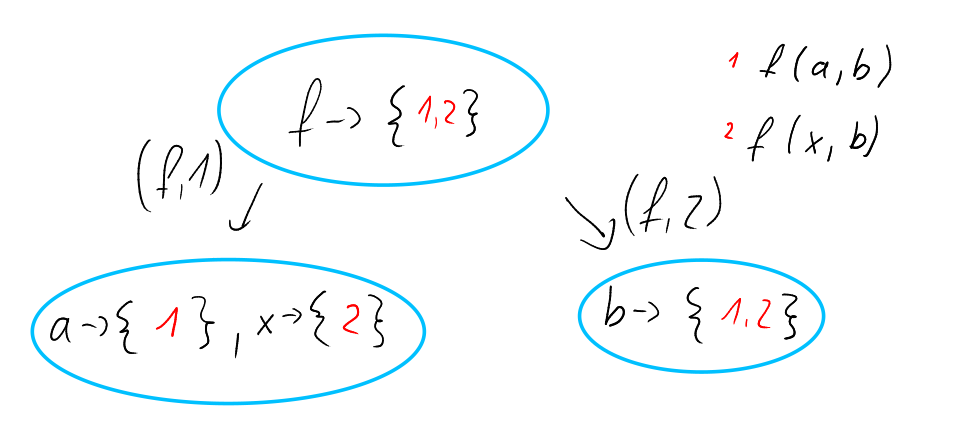
\includegraphics[scale=0.25]{figures/path_index.png}
\caption{A path index}
\label{pathindex}
\end{figure}

We are interested in retrieving the instances, generalisations and unifiables of a term stored in the index. In addition, we define a lookup to retrieve copies of the term. This can be used to check if a term is already contained but may also be of interest as different variables are not distinguished. The queries are based on intersections and unions of the different path sets to enforce constraints on the terms.

To answer the simplest query, the lookup, we procede as follows:
\begin{enumerate}
  \item Compute the set of $(path, symbol)$ pairs describing the term.
  \item Retrieve the path sets corresponding to them in the index.
  \item Intersect the path sets to retrieve all terms containing the same symbols at identical paths as the query term.
\end{enumerate}
  Under the assumption of consistent typing, we retrieve only terms of identical structure as $f(x,y)$ can not exist simultaneously to $f(x)$. Due to the loss of variable identity we may retrieve additional terms.

To retrieve the unifiables of a term from the index, we can use some observations regarding the unification problem.
\begin{enumerate}
  \item A variable is unifiable with any other term
  \item Constants are unifiable with themselves and variables
  \item A function $f(x_{1},...,x_{n})$ is unifiable with term $t$ if and only if $t = x$ or $t = f(y_{1},...,y_{n})$ where for all i $x_{i}$ is unifiable with $y_{i}$. Again, a differing number of arguments are impossible as their types would clash otherwise.
\end{enumerate}
Using this, we can define an algorithm recursing on the structure of the query term while intersecting and unifying the different path sets of the index. The different query types are quite similar, with the lookup being the most restrictive and the unifiables the least restrictive.

$\mathrm{PathTerms(p)}$ refers to the path set stored at the path $p$. $\mathrm{AllTerms}$ is the collection of all terms stored in the index.
\begin{figure}[h]
\centering
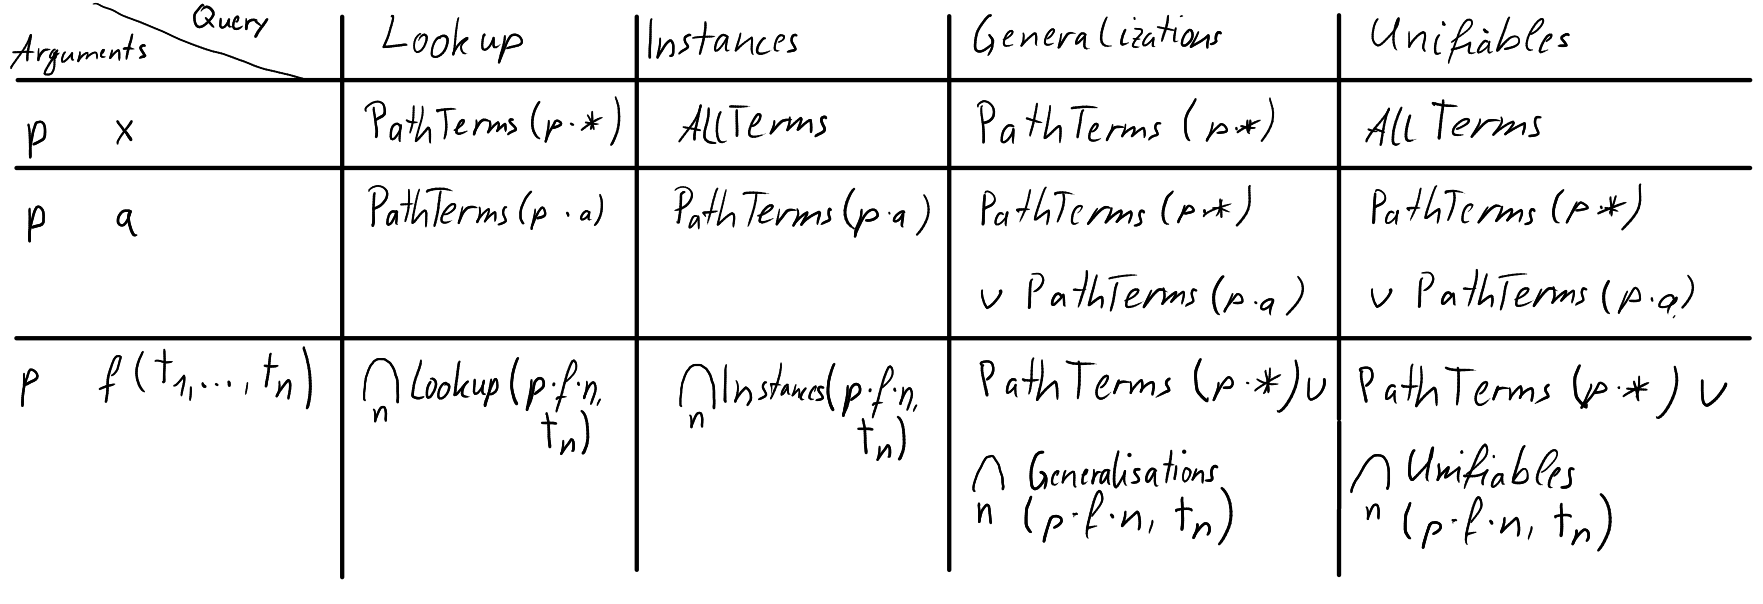
\includegraphics[scale=0.25]{figures/queries.png}
\caption{The different queries and their definition}
\end{figure}

\section{Discrimination Tree}
A discrimination tree index, also known as discrimination net index, is a prefix-sharing tree similar to a trie which stores terms at its leaves and symbols at its internal nodes. To determine the leaf at which a term is stored we use the preorder traversal of the term which we obtain by simply reading the written term from left to right.

\begin{defn}
  $Preorder(t)$ is the sequence of symbols obtained by the preorder traversal of the term $t$. For terminals it is the symbol itself. The preorder traversal of function $f(x_{1},...,x_{n})$ is $<f,Preorder(x_{1}),...,Preorder(x_{n})>$. For the sake of simplicity, we flatten the sequence, i.e. $<f,<g,x>>$ becomes $<f,g,x>$.
\end{defn}
For example, the preorder traversal of $t = f(c,g(x,y))$ is $<f,c,g,*,*>$\footnote{We ignore variable identity as it introduces significant complexity}.

We store the mapping $Preorder(t) \rightarrow t$ in a trie. Due to prefix sharing among the preorders of the different terms this reduces the memory consumption. The leafs contain the terms while the internal nodes only store the symbol by which they are addressed. A discrimination tree storing multiple terms can be seen in \ref{discnet}.

No term is stored in an internal node as, under the assumption of type consistency, it is impossible for $Preorder(t)$ to be a prefix of $Preorder(u)$ if $t \neq u$. If $Preorder(t)$ is a prefix of $Preorder(u)$, $u$ is a combination of $t$ and some other terms. All the functions and their arguments in $t$ are also present in $u$. By the assumption of type consistency, every function present in $t$ is applied to all its arguments and due to the prefix sharing every function in $t$ is also present in $u$ and applied to all its arguments. Thus, $u$ must not consist of any additional terms and therefore be identical to $t$.

\begin{figure}[h]
\centering
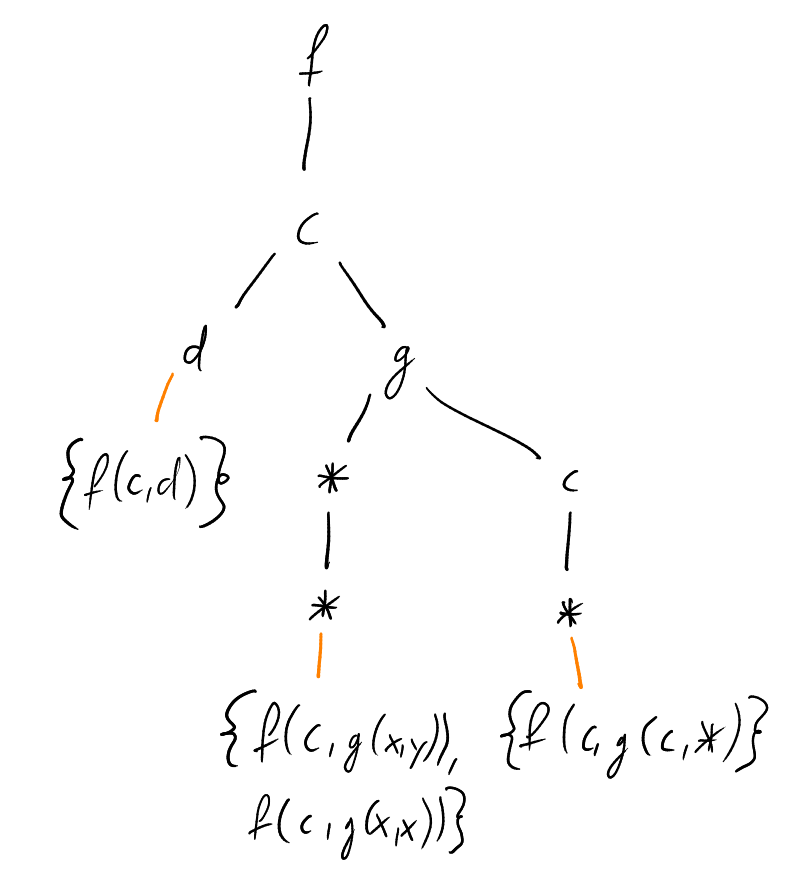
\includegraphics[scale=0.25]{figures/disc_net.png}
\caption{Multiple terms stored in a trie and indexed by the sequence obtained from their preorder traversal}
\label{discnet}
\end{figure}\todo{Root =/= f, besser auf Beispiele ausgelegt: f(c,x) enthalten, netskip kommt vor etc.}

The queries are implemented as a recursive algorithm on the nodes of the trie and $Preorder(t)$ of the query term $t$. Starting at the root, we traverse the tree by selecting the child node corresponding to the first symbol of $Preorder(t)$. We recursively continue at the child node while removing the first symbol from the sequence. In some cases, we may also remove the arguments of the symbol. Therefore, we drop either the first symbol $s$ or $1 + arity(s)$ symbols from the sequence.

\begin{defn}
  $slp(N,c)$ is the symbol lookup operation. It returns the child node of $N$ representing the symbol $c$. If no such node exists, we return the empty node.
\end{defn}

Retrieving the variants of a term is fairly straightforward. Starting at the root, we traverse the trie according to the preorder traversal using $slp$. By doing so, we ensure that we only retrieve terms that contain the same symbols (disregarding variable identity) in the same order, i.e. the variants of the term.

For example, we retrieve the variants of the term $t = f(c,x)$ in the discrimintation tree \ref{discnet} in the following manner, written as $(Node, Preorder(t))$:
$(root, <f,c,x> \rightarrow (f, <c,x>) \rightarrow (c, <x>) \rightarrow (*,<>)$
At this point we have reached a leaf containing the term $f(c,x)$, the only stored variant of the term.

The other queries are more intricate as they may now replace variables by arbitrary terms or symbols by arbitrary terms, with unification allowing both. For every constant symbol in the term we form the union of both the query on the node $slp(N,c)$ aswell as $slp(N,*)$. This ensures that indexed terms containing variables are also retrieved.

A variable in the query term must also be handled differently. As the variable may be replaced by arbitrary terms we must skip a number of nodes depending on the arity of the symbol.
\begin{defn}
  $skip(N)$ returns the set of nodes obtained by skipping a single term starting at $N$. For all symbols $s$ for which $slp(N,s)$ is defined, we collect all nodes $1 + arity(s)$ levels below $N$. That is, for a constant $c$ with $arity(c) = 0$ we return $slp(N,c)$ (which is a direct child of $N$). For a unary function $f$ we return the nodes $slp(slp(N,f),x)$ of all symbols $s$.
\end{defn}
Using this, we can retrieve all the nodes reached by replacing the variable in the query term with some term. The union of the terms returned by the query on each node represents the result. An overview of all the queries is given in \ref{discnetqueries}. Note that $variants$ is the simplest and most restrictive query, $unifiables$ is the most complex and least restrictive with $instances$ and $generalisations$ being a combination of both.

\begin{figure}[h]
\centering
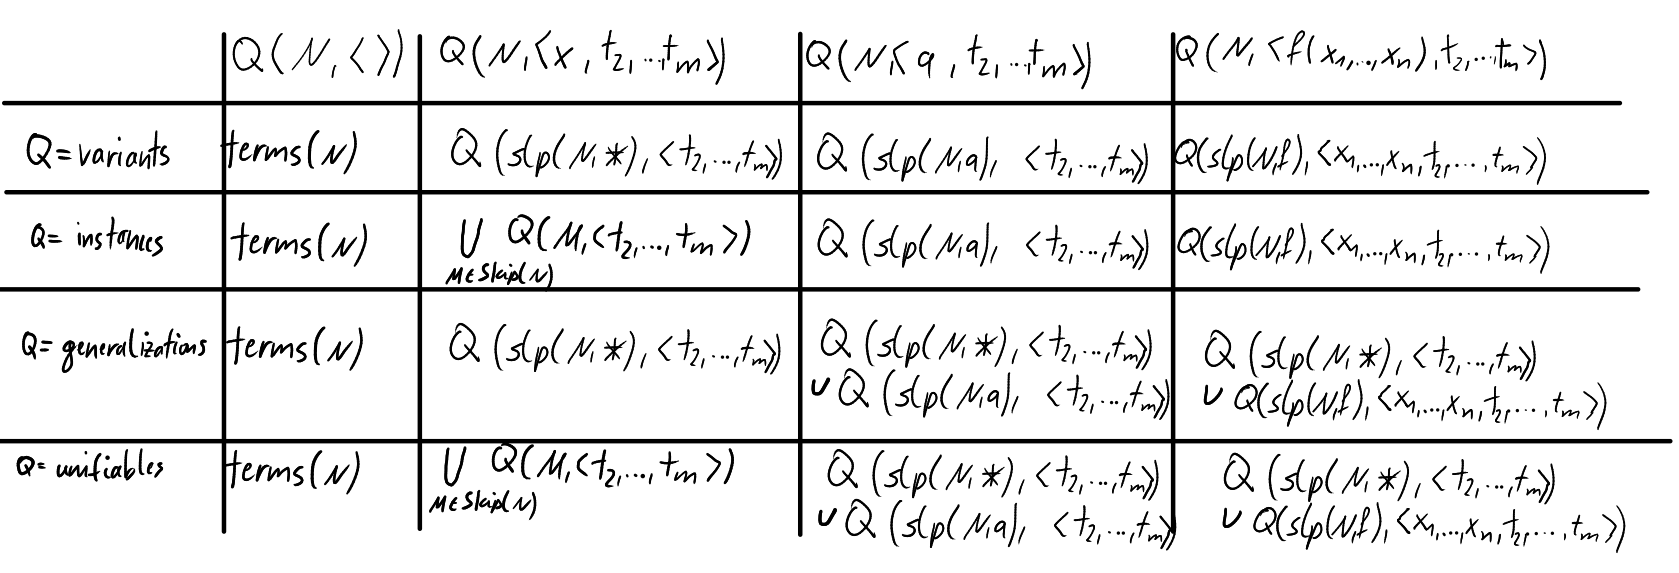
\includegraphics[scale=0.25]{figures/disc_net_queries.png}
\caption{The definition of the different queries}
\label{discnetqueries}
\end{figure}

% \todo{$Symbol_t$ seems completely superfluous, why is it introduced in another paper?}
% \begin{defn}
%   $Symbol_{t}(p)$ refers to the symbol associated with the preorder traversal $p$ of the term $t$ upto the symbol.
% \end{defn}

% For example, the symbols of the term $t = f(c,g(x,y))$ are described by the following mapping:
% \begin{enumerate}
% \item $Symbol_{t}(<>) = f$
% \item $Symbol_{t}(<f>) = c$
% \item $Symbol_{t}(<f,c>) = g$
% \item $Symbol_{t}(<f,c,g>) = *$
% \item $Symbol_{t}(<f,c,g,*>) = *$
% \end{enumerate}

% This mapping can be efficiently stored in a discrimination tree by storing one symbol of the preorder traversal in each internal node and storing

\section{Term Indexing in Isabelle/ML}
As Isabelle has now been used for over 30 years, a number of data structures have already been implemented to store terms. One of the simplest approaches is the \verb!termtable!, a balanced 2-3 tree, storing terms and differentiating them on all attributes, namely their structure, symbols and types. Therefore, this approach is best used when an exact lookup is necessary. On the other hand, \verb!termtables! do not offer any support for the more complex queries.

\subsection{Discrimination Trees}
The need for efficient retrieval of unifiables and generalisations of a query term is addressed by a discrimination tree implementation. Despite being based on the concept introduced above, the discrimination tree implementation in Isabelle/ML stores arbitrary sets of values indexed by terms. This allows us to, for example, store horn clauses for efficient backward chaining. By storing the premises of a clause in the node addressed by its conclusion, we can later query our knowledge base for unifiables of our current goal. On successful retrieval, we can replace the goal with the set of premises.

\begin{figure}[h]
\begin{lstlisting}
  datatype 'a T =
    Leaf of 'a list
  | Net of {atoms: 'a T Symboltable.T, comb: 'a T, var: 'a T}
  val insert: ('a * 'a -> bool) -> term * 'a -> 'a T -> 'a T
  val content: 'a T -> 'a list
  val delete: ('a -> bool) -> term -> 'a T -> 'a T

  val lookup: 'a T -> term -> 'a list
  val instances: 'a T -> term -> 'a list
  val generalisations: 'a T -> term -> 'a list
  val unifiables: 'a T -> term -> 'a list
\end{lstlisting}
\caption{A subset of the signature of the discrmination tree}
\end{figure} \label{discnet_sig}

As we can see from the signature in \ref{discnet_sig}, the discrimination tree stores a list of arbitrary values in each leaf node. The internal nodes, named \verb!Net!, store the children separated into three separate trees. \verb!var! stores both variables and abstractions and atoms stores the constant symbols. Due to the applicative nature of the terms, we also need a \todo{continue here}



The generalisation of storing terms to storing arbitrary single values is relatively simple for discrimination trees but, unfortunately, significantly more difficult for path indexing. This compounds with the fact, that the discrimination tree implementation does not only store arbitrary values but instead efficiently stores sets of arbitrary values. While this does not complicate the datastructre (after all, a data structure for arbitrary values can also store sets of values), the semantics of \verb!insert!, \verb!delete! and duplicate detection are consequently more complicated.

We illustrate this with some examples. We use $(term, value)$ for the items stored and $DT$ for the (initially) empty discrimination tree. We use the syntactic equality although we can avoid deduplication by using a non-reflexive comparsion function:
\begin{enumerate}
  \item Inserting $(a,true)$ and $(b,true)$ into $DT$ stores $true$ at both $a$ and $b$. Retrieving the unifiables of $x$ returns the multiset ${true, true}$ as both $a$ and $b$ are unifiable and the queries do not deduplicate the results.
  \item Inserting $(x,true)$ and $(y,true)$ into $DT$ results in an exception as both are stored in the same node of the tree and the values are identical.
  \item Inserting $(x,x)$ and $(y,y)$ into $DT$ stores both variables $x$ and $y$ in the same node as, by $\alpha$-equivalence, the values are different.\footnote{The term equality used by the discrimination tree to map the higher-order terms to the internal first-order terms without variable identity is not exposed.}
  \item After inserting $(x,true)$ into $DT$, we cannot delete this value without knowing the term used to address the node where the value is stored. Unfortunately, we can delete this value not only with the term $x$ but also with $y$ and $\lambda x. x$ as these are considered to be equivalent by the index. Additionally, deleting a value completely, that is, from all locations it is stored at, is not possible.
\end{enumerate}
The above may not seem too surprising and can be seen as a natural consequence of the design constraints. For example, storing sets of values nicely sidesteps the problem of distinguishing higher-order terms.\todo{Mention mapping of HOL to FOL where?} The discrimination tree can handle higher-order terms without any problems by mapping all \lam -expressions to variables. Therefore, it will return, perhaps extreme, overapproximations to queries but will not fail to store the values or erroneously detect duplication.

The lack of deduplication in queries is a consequence of ease-of-use and consistency. As the insertion of the identical value at different nodes succeeds the different instances of the value should be treated differently. Furthermore, storing the same value multiple times is most likely a rare occurence in which the user is responsible for correct handling.

Nevertheless, this represents significant complexity which, while natural for discrimination trees, must be carefully reproduced in the path index implementation. We recall that a term is never explicitly stored in path indexing as we represent a term by a collection of paths which each store a reference to the term. Naively replacing the reference to the term by a reference to a set of values changes the semantics significantly. Different terms often share at least one path but by no longer storing a reference to the term we lose the information from which term a $(path,value)$ pair originates. Implementing the deletion correctly is no longer possible.
\todo{Continue here}

Unfortunately most literature\todo{2 Quellen sicher, noch welche?} on path indexing only covers the storage of terms. The queries of path indexing rely on the intersection and union of the path sets. These in turn rely on the fast comparison of the stored values. For example, storing hash tables in the path index would be extremely slow as they cannot be compared directly\footnote{The structure of the hashtable depends on the insertion order} and comparing the contents requires the collection of all entries. To solve this potential problem we investigated multiple solutions.

Furthermore, the insertion of an identical $(term,value)$ pair raises an exception. We require a comparison function during insertion to determine this.\footnote{The comparison function need not be reflexive, for example the constant $\mathrm{(\lambda x. false)}$ is valid.} As the index only stores the terms in the path sets we have to store $(term,value)$ pairs in the path sets. Assume we store only the values in the path sets. We cannot determine whether, for example, the path index containing $(f(c),1)$ and $(g(d),1)$ has also stored the $(f(d),1)$ as the value $1$ is present in all path sets associated with $f(d)$, namely $(<>,f)$ and $(<f,1>,d)$.

The first approach requires a comparison function for the values.\footnote{Either as an argument to every function or by implementing path indexing as a functor on a value module} Using the index becomes more difficult by doing so. A user has to implement a comparison function for values and additionally has to consider the potential performance impact. This can be partially mitigated by using $\mathrm{pointerEq}$, although it can only be used as a shortcut for identical values. The comparison must still be called for differing values since there is no perfect sharing.\todo{Code references}\todo{Remove paragraph? Doesn't work with (term,value) pairs}

The second approach is the storage of $(term, value)$ pairs. By doing so we can implement all the operations according to the literature and simply discard the term before returning the results. This simplifies implementation and retains acceptable performance as the comparison of differing terms will likely only need to compare the first few symbols. It will also increase the memory consumption as a copy of every term is stored solely for the set operations. (Additionally there is no immutable pointer implementation in Isabelle/ML\todo{PolyML erwähnen?}. Instead, copies of identical values are shared by the runtime.)\todo{Überhaupt nicht erwähnen weil Data Sharing gut genug funktioniert?}

This approach can be further optimised by replacing the $(term, value)$ pairs by $(identifier, value)$ pairs and mapping each term to an identifier. By using integers as identifier, we reduce the comparison to an integer comparison. Additionally, we can use ordered lists, provided by the SML standard library, for the path sets to implement the set operations more efficiently.\todo{Reference} We are also less reliant on the pointer equality provided by Poly/ML and runtime details like the merging of identical immutable values. This is quite important as we do not have any guarantee when the last heap compression occurred and manual invocation by using the $\mathrm{shareCommonData}$ introduces significant overhead to insertion. Additionally, reliance on low-level functions like $\mathrm{shareCommonData}$ and $\mathrm{pointerEq}$ should be avoided as there are may be significant changes across runtime versions.

We can further speed up the set operations by building a tree of the intersections and unions and only evaluating it at the end. This likely utilizes the cache better because the previously calculated list is not evicted from the cache by the trie traversal. Furthermore, this presumably enables further compiler optimizations as the intermediate results are only short-lived and functions can be inlined. \todo{Example, too vague}

Data Sharing in Poly/ML. NoConstraint exc. No generic hash. Saving ``Copy'' of values because pointers/ref are always mutable and bad for GC etc.

\subsection{Delete Semantics}
There already exists an implementation of a term index in Isabelle/ML with a two caveats. Firstly,
